\documentclass[11pt,twoside,openright]{mpreport}
\usepackage[utf8]{inputenc}
\usepackage[ngerman]{babel}
%\usepackage[T1]{fontenc}
%\usepackage{textcomp}
%\usepackage{mathptmx}
\usepackage[scaled=0.85]{helvet}
%\usepackage{courier}           % if you really want to use Courier
%\usepackage{url}
\usepackage{cite}
\usepackage{tabularx}
\usepackage{amsmath}
\usepackage{amssymb}
\usepackage{hyperref}
\usepackage{ngerman}
\usepackage{wdok-title}
\usepackage{tikz,pgfplots}
\usepackage[section]{placeins} 
\usepackage{here} 
\usetikzlibrary{patterns}
\usetikzlibrary{fpu}
%%\usepackage[pdf]{pstricks}
\setlength{\parindent}{0pt}
\newcommand{\arcosh}{\mbox{arcosh }}
%\pgfplotsset{compat=1.8}
\definecolor{lila}{rgb}{0,0.2,0.8}

% Examples for the definition of convenience commands
\newcommand{\package}[1]{\texttt{#1}}
\newcommand{\foreign}[1]{\emph{#1}}
\newcommand{\q}[1]{»#1«}

% Scale Courier by 0.9
% cf. <http://groups.google.de/groups?selm=yfid76obspu.fsf@triumf.ca>
%\DeclareFontFamily{T1}{pcr}{}
%\DeclareFontShape{T1}{pcr}{m}{n}{
%   <-> s*[.9]pcrr8t
%}{}

\title{Hardware/Software Codesign}
\author{Julian-Benedikt Scholle}
\supervisor{Dr. Ing. Sebastian Zug\\
  Dipl.-Inform Christoph Steup}

\begin{document}
\maketitle
\tableofcontents

\chapter{Einleitung}

\chapter{Anforderungsanalyse}

\chapter{Stand der Technik}

\chapter{Motorstrommessung am Shunt}


\section{Problem}

An einem mit PWM angesteuertem DC-Motor soll eine Strommessung mit Hilfe eines Shuntwiderstandes
durchgeführt werden. Aufgrund der PWM Ansteuerung muss der DC-Anteil aus dem Signal herausgefiltert werden!


\section{Prinzip der Strommessung}

Die Messspannung wird über einen Shuntwiderstand zur Masse gemmessen! Aufgrund nicht vorhandener Datenblätter des Motors
wird von einem Expirimentel Ermittelten maximalen Strom des Motors ausgagangen. Dieser beträgt bei einer Betriebsspannung von 20V ca. 20A.
Da einen Shunt mit einer maximalen Belastbarkeit von 2 Watt eingesetzt wird, darf der maximale Spannungsabfall am Shunt 100mV nicht überschreiten.
Nach dem Ohmschen gesetz ergib sich dadurch ein Widerstand von $0,005 \Omega$  für den Shunt. Shuntwiderstände in der Größe sind problemlos zu bekommen.
Da es sich hir um eine Worst Case Rechnung handelt, wird der zusätliche Widerstand des Shuntwiderstandes und der damit verringerte Strom bewust ignoriert.

Die über den Shuntwiderstand gemessene Spannung soll über den ADC Eingang des Mikrocontrollers eingelesen werden. Vorher jedoch muss das Signal gefiltert werden, da der Strom
durch die Ansteuerung mittels der Pulsweitenmodulation nicht konstant ist!



\section{Anforderungen}
Der maximale Ripple des Endsignals sollte kleiner sein als der Quantisierungsfehler des ADC.\\
Der ADC arbeitet mit einer Auflösung von 10 Bit und einer Referenzspannung von 5V. Der maximale
Ripple $\Delta U_{pp}$ des Endsignals sollte also kleiner sein als $\frac{5V}{1024}=4,88mV$.
Daraus Resultiert eine möglichst hohe Filterordnung bzw. eine niedrige Grenzfrequenz.
$U_{DC}$ soll einer Änderung des Mittelwertes, also einer Änderung des Tastverhältnisses, möglichst
schnell folgen. Diese Anforderung widerspricht der Voherigen so das ein Kompromiss gefunden werden muss.

\section{Dimensionierung des Verstärkers}

In bisherigen Rechnungen wurde ein maximaler Spannungsabfall von 100mV am Shunt errechnet. Da der Messbereich des voll ADC ausgenutzt werden soll,
ist es nötig das Messignal zu verstärken. Hierzu wir ein Nichtinvertierender Verstärker benutzt. Da der Messbereich des ADC bis 5V reicht, wird hier eine 
50 fache Verstärkung angestrebt.

Für einem Nichtinvertierenden Verstärker ergibt sich dann:

\begin{align*}
v &= 1 + \frac{R_2}{R_1}\\
50 &= 1 + \frac{R_2}{R_1}\\
49\cdot R_1 &= R_2
\end{align*}
\\
Wobei z.B. $R_1 = 47 k\Omega$ und $R_2 = 1 k\Omega$  gewählt werden kann, was eine Verstärkung von 48 ergibt






\section{Anforderungen an den Filter}





\begin{figure}[H]
\centering
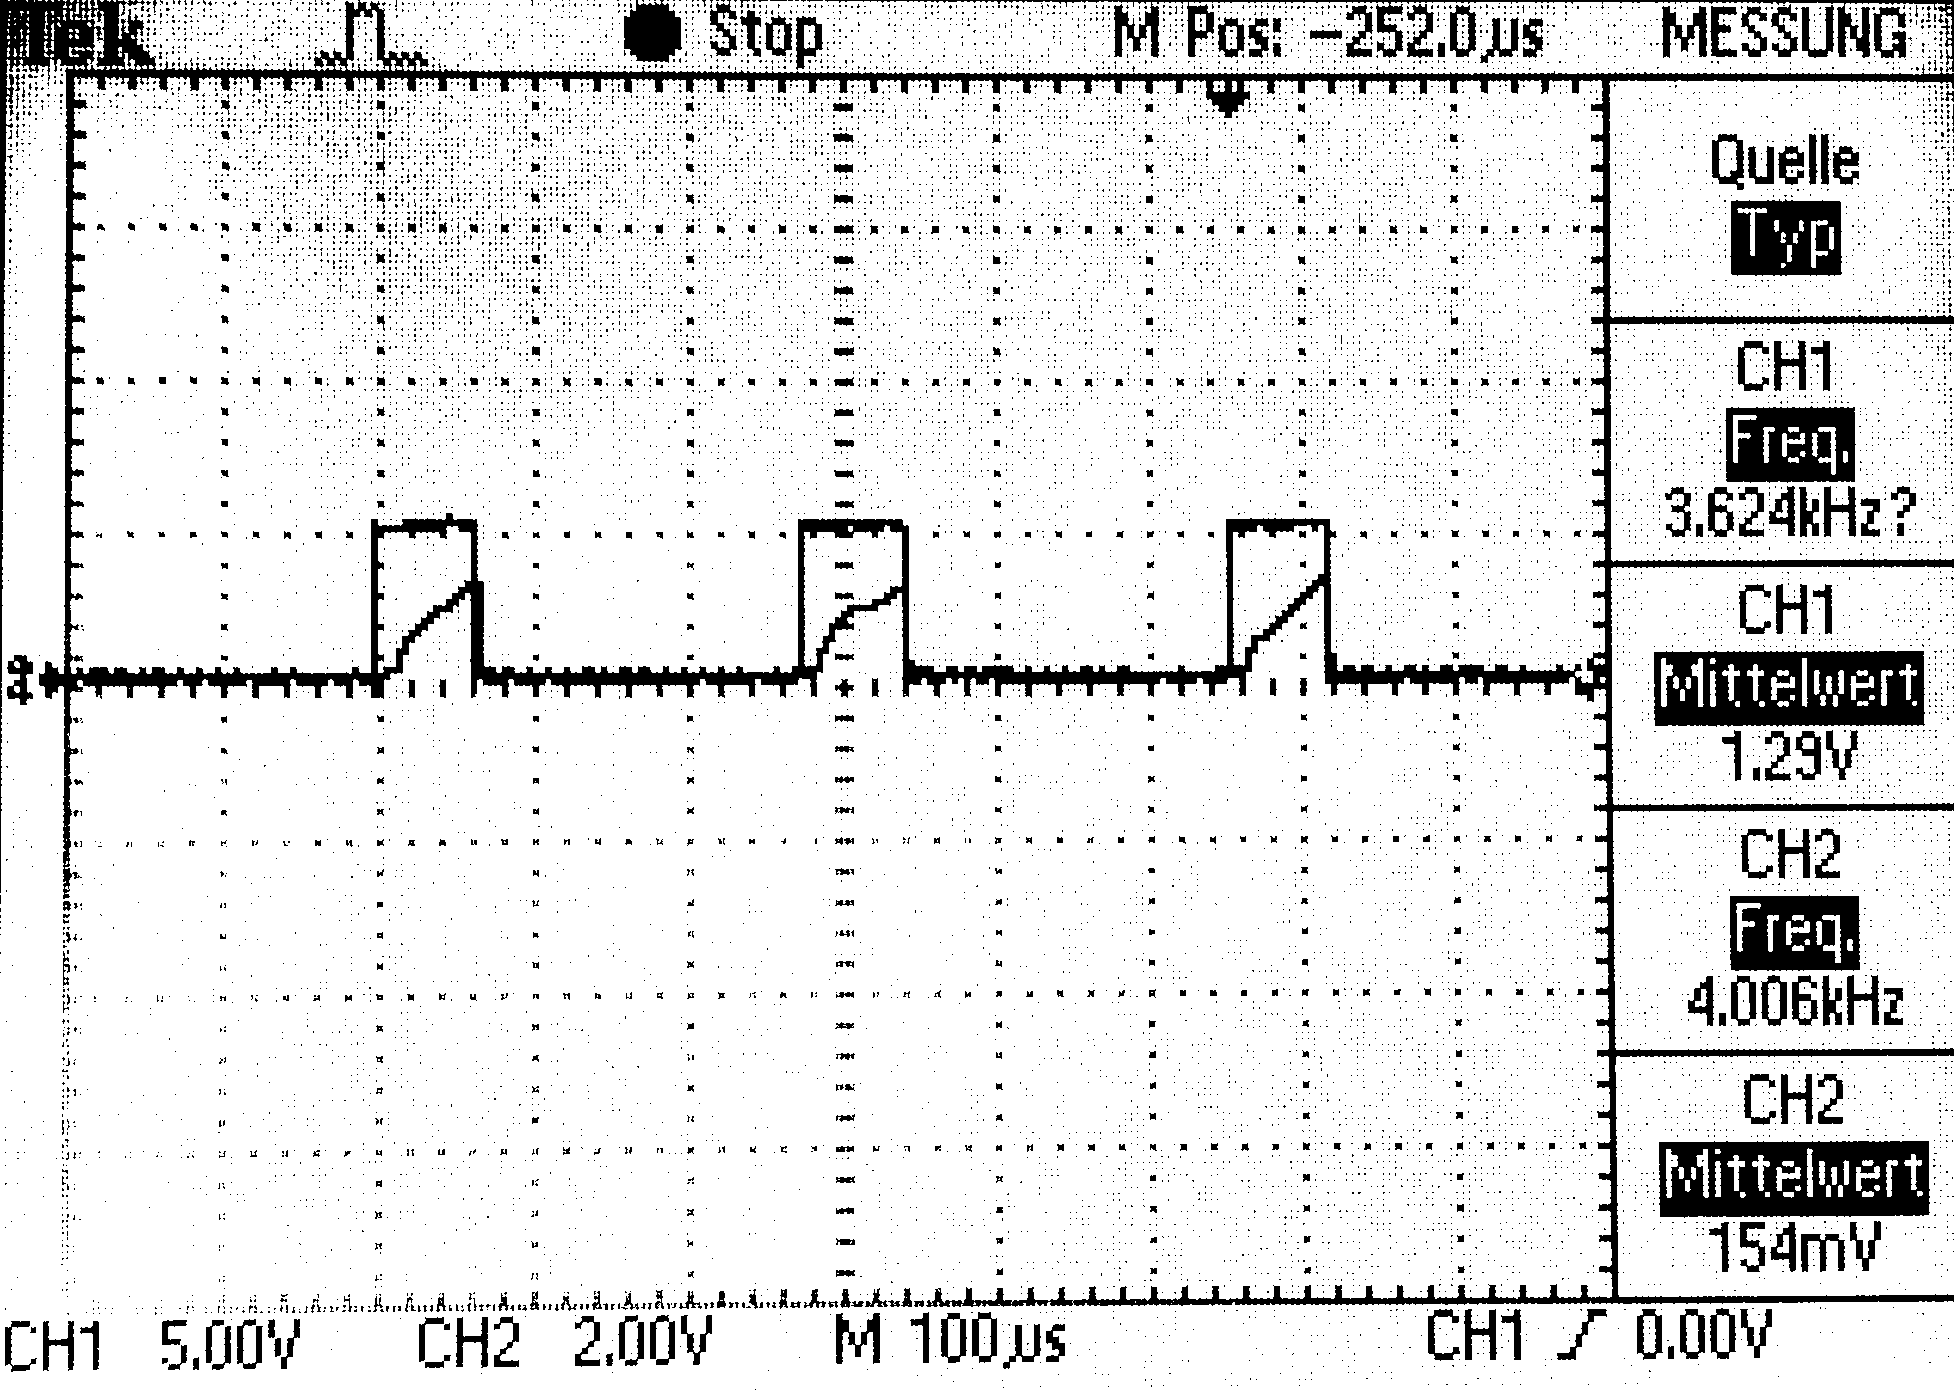
\includegraphics[width=.8\textwidth]{oszi.png}\\
\caption{Spannung am Shunt + PWM}%
\label{fig:pwm+i}
\end{figure}



Da dem Messsignal wie in Abbildung \ref{fig:pwm+i} zu erkennen, die PWM Frequenz zu Grunde liegt wird sich bei der Dimensionierung des Filters einer Idee nach \cite{Alter2008} bedient, nach der die maximale Amplitude des Ripple der Grundschwingung bei einem
Tastverhältnis von 0,5 entspricht. Die Amplitude der Grunschwingung ergibt sich aus dem ersten Koeffizienten der Fouerreihe einer Rechteckschwingung.
\begin{align}
A_1 = K\cdot \frac{1}{\pi}[\sin(\pi p)-\sin(2\pi(1-\frac{p}{2}))]
\label{eq:ripple}
\end{align}
Wobei p dem Tastverhältnis und K der maximale Amplitude des Ursprungsingals entspricht \cite{Alter2008}. K entspricht den erechneten 100mV multipliziert mit dem Verstärkungsfaktor 50, also 5V und p wird zu 0,5
angenommen. Mit (\ref{eq:ripple}) ergibt sich für die Amplitude der Grundschwingung $ A_1 = K\cdot \frac{2}{\pi} = 3,183V$. $A_1$ soll auf $ < 4,88mV$ gedämpft werden.
Als Sperrfrequenz $\Omega_s $ wir hier die PWM Frequenz angesetzt für $H(\omega=2\pi f_{PWM})$ gilt also:

\begin{align}
H(\omega=2\pi f_{PWM}) \le \frac{4,88mV}{3,183V} \mathop{\hat{=}} 20\cdot\log(\frac{4,88mV}{3,183V})= -56,3 dB
\label{eq:daempfung}
\end{align}

Da des Projekt mölicht kostensparend durchgeführt werden soll, also Bauteilsparend, wird an dieser Stelle von den üblichen Konventionen zur dimensionierung von Filtern abgewichen.
Statt eine fixe Grenzfreqeunz festzulegen und die benötigte Filterordnung zu bestimmen, wird die Filterordnung vorgegeben und die Grenzfrequenz variert.

\section{Dimensionierung des Filters}
\begin{figure}[H]
\centering
\begin{tikzpicture}
	\draw[->,thick] (0,0) -- (7.5,0) node[right] {$f[\text{Hz}]$};
	\draw[->,thick] (0,0) -- (0,3.3) node[above] {$a[\text{dB}]$};
	\draw (0,2.5)node[left] {$a_{\text{min}}$} (-0.1,2.5)--(2.9,2.5);
	\draw (0,1)node[left] {$a_{\text{max}}$};
	\def \bsp{(0,1)--(1,1)--(1,2.4)--(1,2.4)--(0,2.4)}
	\draw (-0.1,1)--(1,1)--(1,2.4) (1,0)node[below] {$f_g$};
	\pattern[pattern=north east lines] \bsp;
	\draw[dashed] (1,1) -- (1,-0.1);
	\def \bsd{(3,0) -- (3,2.5) -- (7,2.5) -- (7,0)}
	\pattern[pattern=north east lines] \bsd;
	\draw (3,0)node[below] {$f_s$} -- (3,2.5) -- (7,2.5);

\end{tikzpicture}
\caption{Tiefpass Toleranzfeld}%
\label{fig:analog}
\end{figure}
Für unsere Schaltung wird ein Sallen Key Tiefpass 2. Ordnung entwurfen. Für die PWM-Frequenz $f_{PWM}$ werden 3,9khz angenommen.
Die Sperrfrequenz entspreicht der PWM Frequenz, also der Frequenz unserer Grundschwingung. $\Omega$ entspricht der mit der Grenzfreqeunz 
normierten Frequenz $\Omega=\frac{f}{f_g}$. Nach (\ref{eq:daempfung}) ergibt sich für Abbildung \ref{fig:analog}
$f_s=f_{PWM}=3,9 kHz$, $a_{min}=56,3 dB$ und $a_{max}$ wird auf 3dB festgelegt.



\subsection{Butterworth}
\subsection{Bestimmung der Grenzfreqeunz}
\begin{align}
n \ge \frac{\log{\sqrt{\frac{e^{2a_{min}}-1}{e^{2a_{max}}-1}}}}{\log{\Omega_s}}
\label{eq:butterworth}
\end{align}
Die Filterordnung nach Butterworth wird nach (\ref{eq:butterworth}) bestimmt. Umgestellt nach $\Omega_s$ ergibt sich:

\begin{align}
\Omega_s \le  \left(\frac{e^{2a_{min}}-1}{e^{2a_{max}}-1}\right)^{\frac{1}{2n}}
\end{align}



Für die Berechnung der Sperrfrequenz $\Omega_s$ müssen  $a_{min}$ und $a_{max}$ in Neper umgrechnet werden. Wobei:
\begin{align*}
1 \text{dB} =  \frac{\ln{10}}{20}\text{Np} = 0,115129255 \text{Np}   
\end{align*}

Damit ergibt sich für $a_{min}=56,3 dB\cdot \frac{\ln{10}}{20}=6,48Np$ und für  $a_{max}=3 dB\cdot \frac{\ln{10}}{20}=0,345Np$. Die Filterordnung wird auf 2 festgelegt.
\begin{align}
\Omega_s \le  \left(\frac{e^{2\cdot6,48N }-1}{e^{2\cdot 0,345Np}-1}\right)^{\frac{1}{2n}}  = 35,8
\end{align}

Die Grenzfreqeunz $f_g$ ergibt sich jetzt aus:

\begin{align}
\frac{f_s}{\Omega_s} \le \frac{3,9kHz}{35,8} = 108,8Hz
\end{align}

\subsubsection{Filterentwurf}
Im voherigen Abschnitt wurde berechnet das die Grenzfreqeunz der Filters kleiner als 108,8Hz sein muss.
Im Folgenden wird nun ein Sallen-Key Filter 2. Ordnung mit einer Grenzfrequenz von 100Hz entwurfen.

\begin{figure}[H]
\centering
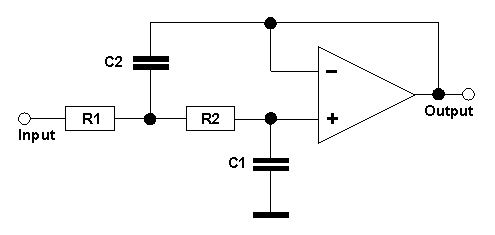
\includegraphics[scale=0.8]{tiefpass_sk.png}\\
\caption{Sallen-Key Tiefpass}%
\label{fig:tiefpass_sk}
\end{figure}
Die Allgemeine Filterübertragungsfunktion lautet:
\begin{align}
A(P)=\frac{A_0}{1+c_1P+c_2P^2+...+C_nP^2}
\label{eq:pass_alg}
\end{align}


Die Übertragungsfunktion eines Sallen-Key Tiefpasses lautet:
\begin{align*}
A(P)&=\frac{1}{1+\omega_g (R_1 C_1 + R_2 C_1)P + \omega_g^2R_1 R_2 C_1C_2P^2}
\end{align*}
Zur vereinfachung setzen wir $R_1 =R_2=R$. Die Übertragungsfunktion lautet dann:
\begin{align}
A(P)&=\frac{1}{1+2\omega_g RC_1P+\omega_g^2R^2C_1C_2P^2}
\label{eq:pass_sk}
\end{align}


Mit (\ref{eq:pass_alg}) und (\ref{eq:pass_sk}) ergeben sich die Filterkoeffizienten. 
Sie lassen sich nach Butterworth ($a_{max}=3dB$) den üblichen Tabellen
entnehmen und müssen nicht extra brechnet werden. Sie lauten für einen Filter 2. Ordnung:

\begin{minipage}{0.5\textwidth}
\begin{align*}
c_1 &= 2\omega_g R C_1\\
c_1 &= 1,4142
\end{align*}
\end{minipage}
\begin{minipage}{0.5\textwidth}
\begin{align*}
c_2&=\omega_g^2 R^2 C_1 C_2\\
c_2&= 1
\end{align*}
\end{minipage}
\\

Nun werden die Filterkoeffizienten nach den Kapazitäten aufgelöst. R ist dabei frei wählbar und wird auf 1$k\Omega$ gesetzt

\begin{minipage}{0.5\textwidth}
\begin{align*}
  c_1&= 2\omega_g R C_1\\
  C_1&=\frac{c_1}{2\omega_g R}\\
  C_1&=\frac{1,4142}{4\pi \cdot 100\text{Hz} \cdot1000\Omega}\\
  C_1&=1,125\mu\text{F}
\end{align*}
\end{minipage}
\begin{minipage}{0.5\textwidth}
\begin{align*}
  c_2&=\omega_g^2 R^2 C_1 C_2\\
  C_2&=\frac{c_2}{\omega_g^2 R^2C_1}\\
  C_2&=\frac{1}{(2\pi \cdot 100\text{Hz})^2 \cdot 1000^2\Omega \cdot 1,125\mu\text{F}}\\
  C_2&=2,25\mu\text{F}
\end{align*}
\end{minipage}
\\

Kondensatoren die den Größen am ehesten entsprechen sind $1,2\mu\text{F}$ und $2,2\mu\text{F}$, weshalb diese Größen für die Nachfolgende Simulation genutzt werden.
\subsubsection{Simulation}
Für die Simulation der Schaltung wurden Ideale Operationsverstärker verwendet.
Das Testsignal ist eine Rechteckschwingung mit dem Tastverhältnis 0,5 und einer Frequenz von 3,9kHz.
\begin{figure}[H]
\centering
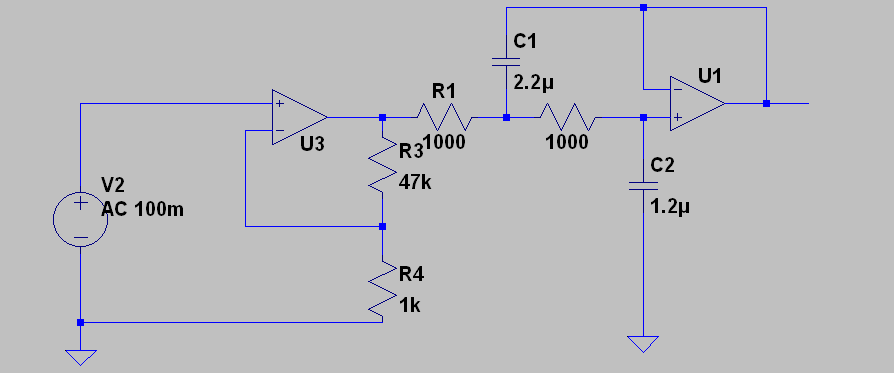
\includegraphics[width=.96\textwidth]{schaltung.png}\\
\caption{Schaltung in LT-Spice}%
\label{fig:tp-schaltung}
\end{figure}



\begin{figure}[H]
\centering
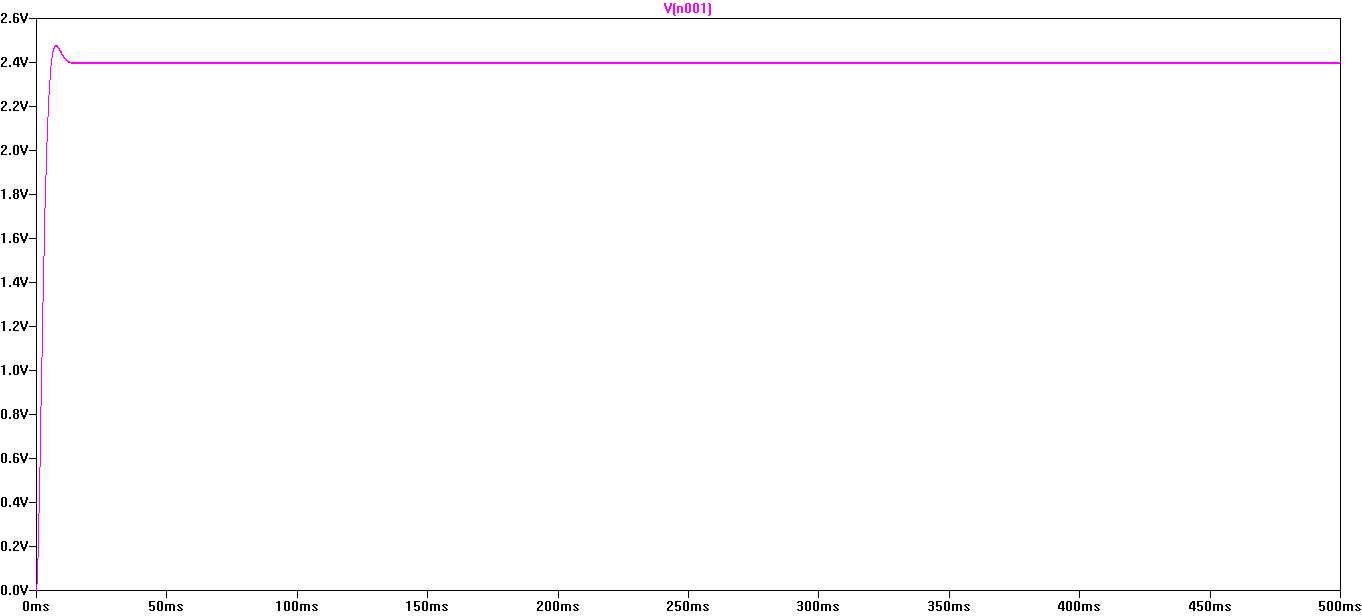
\includegraphics[width=.96\textwidth]{plott.png}\\
\caption{Simulationsergebnis des Butterworth-Filters}%
\label{fig:tp-plott-bw}
\end{figure}

Wie man am Folgenden Diagramm sehen kann liegt der Ripple unter den geforderten 4,88mV, bei ca 3,3mV und entspticht damit den Anforderungen


\begin{figure}[H]
\centering
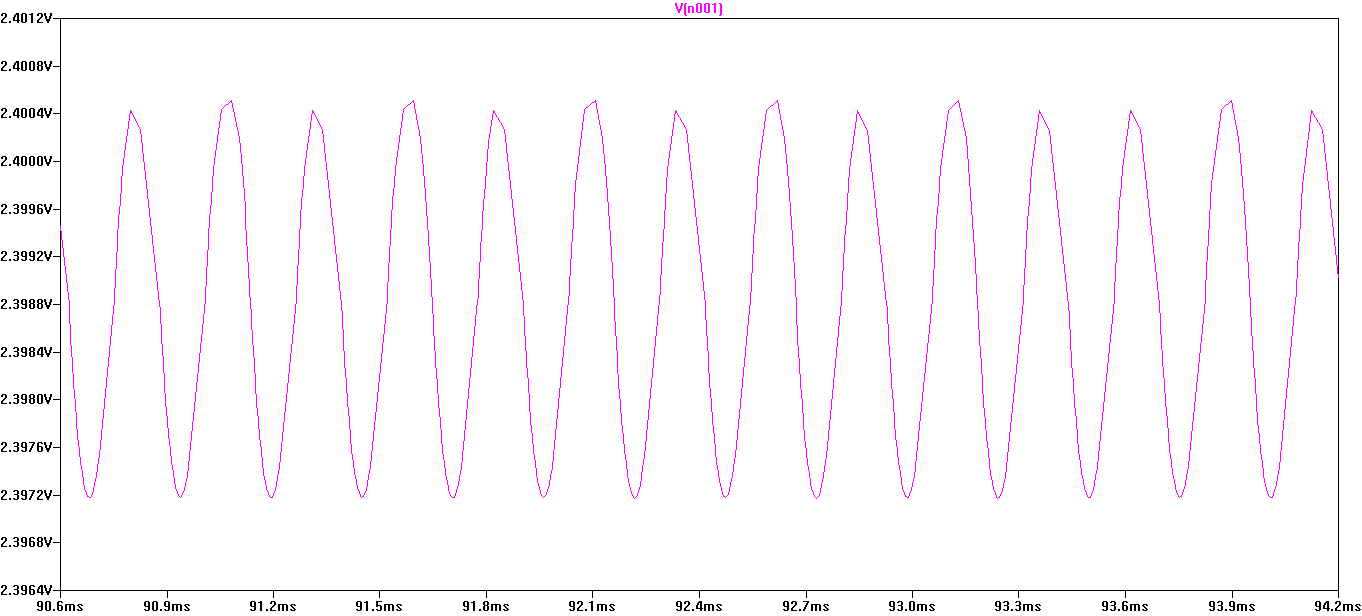
\includegraphics[width=.96\textwidth]{ripple.png}\\
\caption{Ripple des Butterworth-Filters}%
\label{fig:plott_ripple-bw}
\end{figure}



\subsection{Tschebyscheff}

\subsubsection{Bestimmung der Grenzfreqeunz}


\begin{align}
n \ge \frac{\arcosh{\ln{\sqrt{\frac{e^{2a_{min}}-1}{e^{2a_{max}}-1}}}}}{\arcosh \ln{\Omega_s}}
\label{eq:tschebyscheff}
\end{align}

Die Filterordnung nach Tschebyscheff wird nach (\ref{eq:tschebyscheff}) bestimmt. Umgestellt nach $\Omega_s$ ergibt sich:

\begin{align}
\Omega_s \le \exp{\left(\cosh{\left(\frac{\arcosh{\ln{\sqrt{\frac{e^{2a_{min}}-1}{e^{2a_{max}}-1}}}}}{n}\right)}\right)}
\end{align}


Für die Berechnung der Sperrfrequenz $\Omega_s$ müssen  $a_{min}$ und $a_{max}$ wieder Neper umgrechnet werden.
Es ergibt sich für $a_{min}=56,3 dB\cdot \frac{\ln{10}}{20}=6,48Np$ und für  $a_{max}=3 dB\cdot \frac{\ln{10}}{20}=0,345Np$. Die Filterordnung wird erneut auf 2 festgelegt.


\begin{align}
\Omega_s \le \exp{\left(\cosh{\left(\frac{\arcosh{\ln{\sqrt{\frac{e^{2\cdot 6,48Np}-1}{e^{2\cdot 0,345Np}-1}}}}}{2}\right)}\right)} = 6,92
\end{align}



Die Grenzfreqeunz $f_g$ ergibt sich jetzt aus:

\begin{align}
\frac{f_s}{\Omega_s} \le \frac{3,9kHz}{6,92} = 563,6Hz
\end{align}


\subsubsection{Filterentwurf}
Im voherigen Abschnitt wurde berechnet das die Grenzfreqeunz der Filters für eine Tschebyscheff abstimmung kleiner als 563,6Hz sein muss.
Im Folgenden wird nun ein Sallen-Key Filter 2. Ordnung mit einer Grenzfrequenz von 550Hz entwurfen.

\begin{figure}[H]
\centering
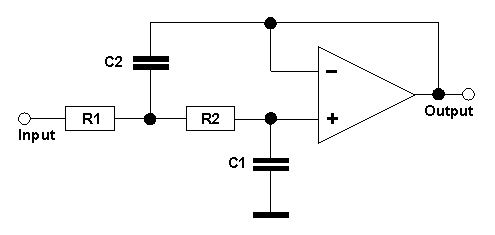
\includegraphics[scale=0.8]{tiefpass_sk.png}\\
\caption{Sallen-Key Tiefpass}%
\label{fig:tiefpass_sk}
\end{figure}

Mit (\ref{eq:pass_alg}) und (\ref{eq:pass_sk}) ergeben sich die Filterkoeffizienten. 
Sie lassen sich nach Tschebyscheff ($a_{max}=3dB$) den üblichen Tabellen
entnehmen und müssen nicht extra brechnet werden. Sie lauten für einen Filter 2. Ordnung:

\begin{minipage}{0.5\textwidth}
\begin{align*}
c_1 &= 2\omega_g R C_1\\
c_1 &= 0,91082
\end{align*}
\end{minipage}
\begin{minipage}{0.5\textwidth}
\begin{align*}
c_2&=\omega_g^2 R^2 C_1 C_2\\
c_2&= 1,41279
\end{align*}
\end{minipage}
\\

Nun werden die Filterkoeffizienten nach den Kapazitäten aufgelöst. R ist dabei frei wählbar und wird auf 1$k\Omega$ gesetzt

\begin{minipage}{0.5\textwidth}
\begin{align*}
  c_1&= 2\omega_g R C_1\\
  C_1&=\frac{c_1}{2\omega_g R}\\
  C_1&=\frac{0,91082}{4\pi \cdot 550\text{Hz} \cdot1000\Omega}\\
  C_1&=0,1317\mu\text{F}
\end{align*}
\end{minipage}
\begin{minipage}{0.5\textwidth}
\begin{align*}
  c_2&=\omega_g^2 R^2 C_1 C_2\\
  C_2&=\frac{c_2}{\omega_g^2 R^2C_1}\\
  C_2&=\frac{1,41279}{(2\pi \cdot 550\text{Hz})^2 \cdot 1000^2\Omega \cdot 0,1317\mu\text{F}}\\
  C_2&=0,898\mu\text{F}
\end{align*}
\end{minipage}
\\

Kondensatoren die den Größen am ehesten entsprechen sind $0,82\mu\text{F}$ und $0,12\mu\text{F}$, weshalb diese Größen für die Nachfolgende Simulation genutzt werden.
\subsubsection{Simulation}
Die Schaltung entspricht die der Simulation für einen Butterworth-Filter
Das Testsignal ist eine Rechteckschwingung mit dem Tastverhältnis 0,5 und einer Frequenz von 3,9kHz.
\begin{figure}[H]
\centering
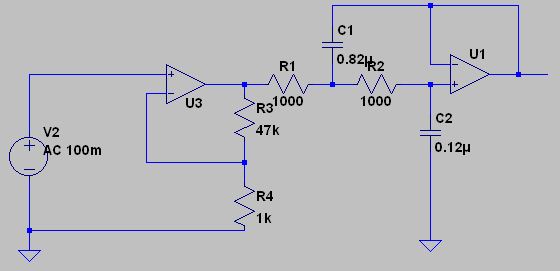
\includegraphics[width=.96\textwidth]{schaltung_ts.png}\\
\caption{Schaltung in LT-Spice}%
\label{fig:tp-schaltung_ts}
\end{figure}



\begin{figure}[H]
\centering
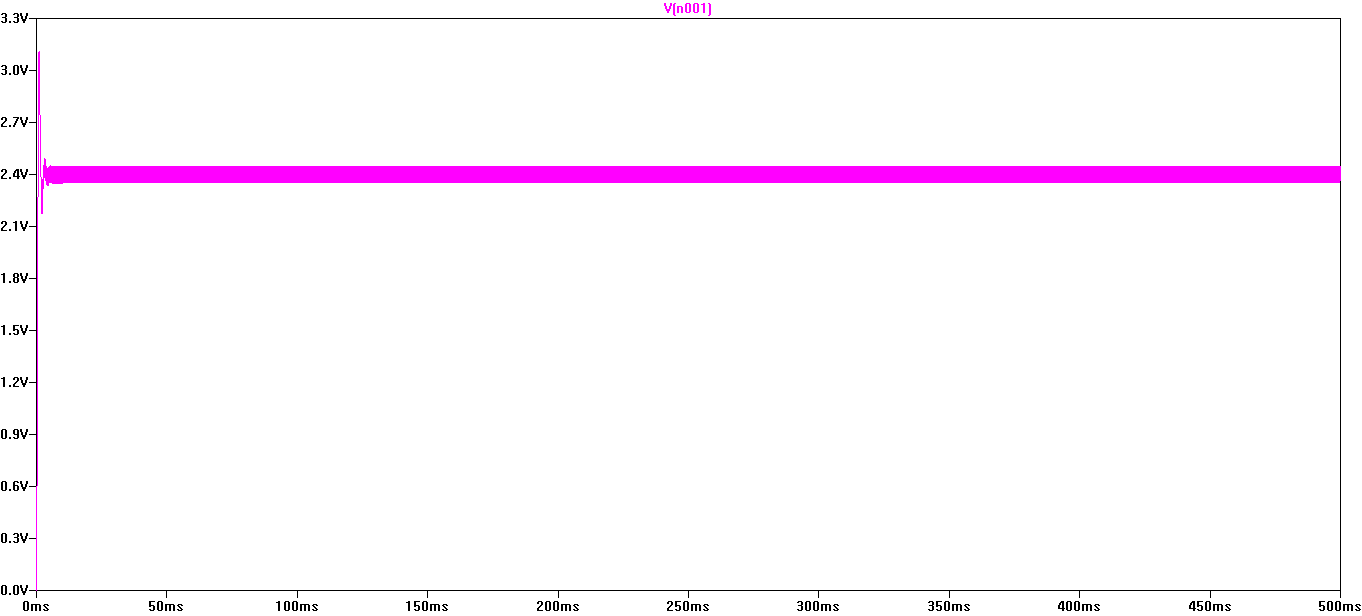
\includegraphics[width=.96\textwidth]{plott_ts.png}\\
\caption{Simulationsergebnis des Tschebyscheff-Filters}%
\label{fig:tp-plott-ts}
\end{figure}

Wie man am Folgenden Diagramm sehen kann liegt der Ripple weit über den geforderten 4,88mV  und entspticht damit nicht Anforderungen, sodas
der Tschebyscheff-Filter ind dieser Form nicht führ unsere Anwendung geeignet ist. Eventuell würde ein keineres $a_{max}$ ein besseres Ergebniss
liefen. Da die Abstimmung nach Butterworth jedoch den Anforderungen bereits genügt wird an dieser Stelle darauf verzichtet.

\begin{figure}[H]
\centering
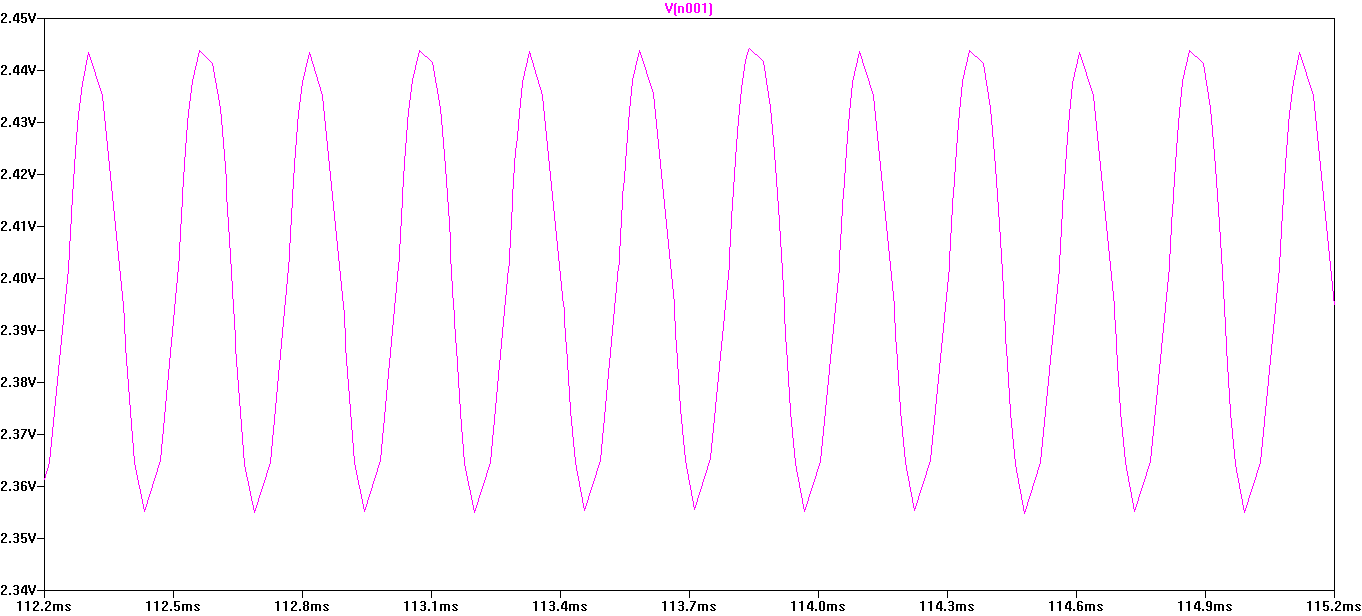
\includegraphics[width=.96\textwidth]{ripple_ts.png}\\
\caption{Ripple des Tschebyscheff-Filters}%
\label{fig:plott_ripple-ts}
\end{figure}


\subsubsection{Finaler Entwurf}
Übertragungsfunktion eines Sallen-key Teifpasses
\begin{align*}
A(P)&=\frac{A_0}{1+\omega_g (R_2 C_2 + R_1 C_2 + R_1 C_2(1-A_0))P + \omega_g^2R_1 R_2 C_1C_2P^2}
\end{align*}

mit
\begin{align*}
A_0=\frac{R_6}{R_5}-1
\end{align*}


Die Bauteilwerte erhält man durch einen Koeffizientenvergleich mit der entnormierten
Übertragungsfunktion eines Tiefpasses zweiter Ordnung:

\begin{align*}
A(P)&=\frac{A_0}{1+\frac{1}{\omega_g\Omega_PQ_P}s+\frac{1}{\omega_g^2\Omega_P^2}s^2}
\end{align*}



\bibliography{BIB}{}
\bibliographystyle{plain}

\end{document}